\documentclass[a4paper]{article}

\usepackage[swedish]{babel}
\usepackage[T1]{fontenc}
\usepackage[utf8]{inputenc}
\usepackage{graphicx}
\usepackage{makecell}
\setlength\parindent{0pt} %changes indentation size to 0

\begin{document}

\title{
  Projektplan DAT290 \\
  \large MD407 Säkerhetssystem, Grupp 13}
\date{2020-09-07}

\author{Sebastian Sjögren, Gabriel Käll, Philip Antonsson, \\ Erik Nilsson, Simon Widerberg, Felix Bråberg \\ Linus Haraldsson}

\maketitle
\thispagestyle{empty}
\newpage

\tableofcontents
\thispagestyle{empty}
\newpage
\pagenumbering{arabic}

%Ni skriver all text i projektplanen med ett projektinternt perspektiv.
%Detta betyder att ingenstans ska det framgå att projektet drivs inom
%ramen för en kurs i utbildningssyfte, utan att detta är ett renthttps://www.overleaf.com/project/5f5652a06c50130001db661f
%tekniskt utvecklingsprojekt.

%Eftersom de tre första avsnitten, Syfte, Mål och Bakgrund, återkommer
%(helt intakta, om de är välskrivna) i projektrapporten, tveka inte över
%att ägna ordentligt med tid åt dessa.


\section*{Ordlista}
\label{sec:ordlista}
\begin{description}
    \item[USART]{Universal Synchronous/Asynchronous Reciever/Transmitter är en periferienhet som omvandlar data till bitströmmar. Används för att möjliggöra kommunikation mellan två hårdvaruenheter.}\cite{howe:2020}
    \item[CAN]{Ett asynkront protokoll för kommunikation mellan separata hårdvaruenheter.}  \cite[pg 249]{lme:2016}
    \item[GitHub]{Webbhotell för lagring sin källkod öppet.}
    \item[Branch]{En version av mjukvara som lagras på Github.}
    \item[Pulla]{Att ladda ned en viss specificerad version av ett program från Github eller något annat webbhotell.}
    \item[Pusha]{Att ladda upp sin version av ett program till Github eller något annat webbhotell.}
    \item[Structs]{En datastruktur, d.v.s. en bit av bestämt minne i datorn där data är grupperat och lagrat för lätt åtkomst.}
    \item[IO]{Input-Output, representerar in- och utmatning av data.}
    \item[Discord]{En plattform för gruppsamtal över internet.}
\end{description}

\section{Syfte}
\label{sec:syfte}


%Syftet beskriver koncist varför projektet ska genomföras och vad ett
%uppfyllande av de tekniska målen leder till.

%Vanligtvis är syftet så klart ledande för uppgiften man löser. Här är
%det lite tvärt om eftersom ni fått en uppgift och måste komma på ett
%syfte för den, men det ska nog gå bra.

%Ha gärna med lite fakta i syftesparagrafen. Istället för att bara skriva
%självklarheter som att det är bra med larm ifall det kommer tjuvar så
%kan man ha med några siffror på vad larmbranchen omsätter till exempel
%eller hur vanligt det är med inbrott eller något.
Syftet med projektet är att utföra och dokumentera skapandet av ett lås- och larmsystem. År 2018 var det cirka 82 000, eller 1,8 procent, av rikets hushåll som rapporterade fall av bostadsinbrott i Sverige. Detta antal är detsamma år 2016 och 2017\cite{ntu:2019}. Därmed är det viktigt att säkra larm- och låssytem finns till för medborgares säkerhet. Larmsystemet skall vara utmanande att bryta sig igenom.


\section{Mål}
\label{sec:mål}
%I detta avsnitt beskrivs koncist samtliga övergripande tekniska mål med
%projektet, det vill säga, vad ska konstrueras. Mycket av det här
%framgår så klart i uppgiften.

%Se till att tydligt ange målsättningen vad gäller de extrauppgifter som
%finns tillgängliga i projektdirektiven. Ni kan dela upp eventuella
%extrauppgifter i två olika prioritetsgrader. Att ta på sig en massa
%extrauppgifter här som ni inte ens försöker genomföra är inte bra.
%Försök göra en realistisk bedömning av vad ni hinner med även om det är
%svårt.

%De mål som anges här kommer att styra projektets utveckling. När
%projektet närmar sig sitt slut och den slutliga projektrapporten lämnas
%in kommer beställaren (läraren i vårt fall) att kritiskt analysera hur
%väl projektet lyckats genom att jämföra planens mål med den tekniska
%konstruktion som redovisas i projektrapporten.

Målet med projektet är att skapa ett larm- och låssystem med hjälp av en centralenhet tillsammans med 2 periferienheter och en störenhet. Alla enheter ska ha sina isolerade funktioner och uppgifter. De två periferienheterna är ett dörrlarm och ett rörelselarm. Övergripligt ska periferienheterna larma till centralenheten medan störenheten är till för att stresstesta systemet. Alla delsystem skall samarbeta för att tillsammans skapa ett fungerande larm- och låssystem.
\newline\newline
Två utökningar av grundsystemet är planerade. Den ena är att rörelselarmet inte skall larma till centralenheten förrän det befinner sig någon inom en viss variabel räckvidd från enheten. Alltså skall rörelselarmet endast larma lokalt tills räckvidden blir överskriden av någon. Den andra planerade utökningen är att ljudet som uppgör larmet sticker ut och är så tydligt som möjligt. Prioriteringen av utökningarna är i samma ordning som de introducerades ovan.


\section{Bakgrund}
\label{sec:bakgrund}

%Genom att det fyller i de kompetensluckor som en typisk läsare har,
%underlättar bakgrundstexten läsandet av konstruktionsavsnitten. Precis
%som avsnitten Syfte och Mål ovan kan detta avsnitt med fördel
%återanvändas i den slutgiltiga projektrapporten. När det gäller
%projektplanen för DAT290 beskrivs här bakgrunden till projektet vad
%gäller tillämpningen, dess sammanhang och de tekniska förutsättningar
%som råder. För att beskriva tillämpningen och dess sammanhang behöver ni
%förklara hur system av den typen som ska konstrueras här fungerar i
%största allmänhet.

%Men vem är den typiska läsaren? Man får förutsätta att läsaren har en
%viss teknisk kompetens, annars blir bakgrundsavsnittet alltför långt.
%Denna gränsdragning (“hur elementärt ska jag förklara vad jag gör?”)
%upplevs som ett svårt moment när man som student börjar skriva tekniska
%rapporter. En användbar regel är att vi utgår från att läsaren har, i
%stort sett, samma utbildning som rapportskribenten, men saknar
%specialistkunskap om projektets tillämpning.


Alla larmsystem är olika, men de flesta innehåller dessa huvuddelar: 
\begin{enumerate} 
    \item Sensorer
    \item Centralutrustning 
    \item Larmdon (Larmenhet)
    \item Larmsändare (Överför fel/larm till ev. mottagare)
    \item Förbikopplare (Möjliggör modularitet i larmsystemet)
    \item Strömförsörjning
\begin{flushright}
   \cite[pg 15]{lundh:2008}
\end{flushright}

\end{enumerate}
Alla dessa komponenter sammanvävs till ett larmsystem, där sensorerna agerar som larmsystemets ''sinnen'', och centralenheten (Centralutrustningen) som systemets ''hjärna''. 
I allmänhet fungerar larmsystem som liknar det som ska skapas såhär:

\begin{enumerate}
 \item Det finns en centralenhet som är kopplad till ett antal moduler. Modulerna är ofta sensorer, stömbrytare eller fysiska/virtuella gränssnitt för användaren. Sensorerna detekterar ändringar i tillstånd och notifierar centralenheten.


 \item Centralenheten tar emot information från modulerna. Regelbunden information är väsentlig eftersom centralenheten behöver veta om en enhet plötsligt blir frånkopplad - att ett inbrott/problem har förekommit.
 \item För att enheterna ska kunna kommunicera behövs antingen en trådad eller trådlös anslutning, men för enkla system används ofta en databuss. Dessa kan vara bra ur en ekonomisk synpunkt. \ \cite[pg 16, pgrph 2]{lundh:2008} Men enheterna behöver inte bara kunna kommunicera - de behöver kunna kommunicera effektivt. Därför behövs ett system som prioriterar viktiga meddelanden och undviker kollisioner. 
 
\end{enumerate}
\newpage
\subsection{Tekniska förutsättningar}
\label{sec:tekniska förutsättningar}

I projektet kommer det användas diverse hårdvara, varav majoriteten är given från början. Den givna hårdvaran är allt som involverar gränssnittet mellan användare och system, samt kommunikation mellan externa moduler och centralenheten.
\newline
\newline
Resten av hårdvaran ska utvecklas löpande under projektet med hjälp av en kopplingsplatta. Anledningen varför ytterligare hårdvara behöver utvecklas är huvudsakligen för att avståndsmätaren och vibrationssensorn annars inte kan kopplas till systemet. Vi behöver utforma kretsar åt dessa sensorer som leder till att centralenheten får en klar signal när dessa triggas. Utöver det kommer kopplingsplattan användas för att simulera verkligheten. En strömbrytare kan agera som en öppen eller stängd dörr och lysdioder/ljudsignaler används för att enkelt signalera till oss när alarmet (lokalt eller globalt) har utlösts. 
\newline
\newline
Projektet kodas i C, med hjälp av CodeLite. Det kommer skapas ett CodeLite-projekt för varje modul, och vid körning exporteras projektkoden till respektive modul.
För att abstrahera bort svårskriven lågnivåkod används ''STM32F4xx Standard Pheripherals Library''. Det är ett bibliotek för processorn i laborationsenheten MD407, och underlättar initiering och användning av olika kommunikationstyper som kortet stödjer. 
\newline
\newline
Den kod som behöver nyutvecklas är en viktig del av systemet, nämligen kommunikationsprotokollet som tillämpas mellan enheterna. Enheterna kommer vara ihopkopplade med hjälp av en CAN-buss. CAN är ett asynkront protokoll som används omfattande i industriell automation, och för kommunikation mellan mikroprocessorer i moderna bilar. \cite[pg 249]{lme:2016} Med andra ord, ett välgrundat protokoll. 
\newline \newline
Det som behöver implementeras är en meddelandestruktur modulerna kan förhålla sig till. Vi behöver därmed definera vilken data som ska skickas inuti alla typer av CAN-meddelanden, och hur datan ska tolkas av andra enheter. Det behövs också kod som gör att centralenheten kan få information från användare. Både på hårdvarunivå genom knappsatsen och mjukvarunivå, genom ett konsollfönster på användarens dator, USART.

%När det gäller tekniska förutsättningar så behöver ni förtydliga vad som
%är givet i projektet: Beskriv övergripande vilken hårdvara och mjukvara
%som kan förutsättas och vad som ska nyutvecklas. Som ni senare kommer
%upptäcka överlappar denna beskrivning till viss del med resursplanen i
%avsnitt \ref{sec:resursplan}. I och med att detta sista avsnitt skiljer sig
%ganska mycket från tillämpningsgenomgången ovan kan det här vara läge
%att använda sig av en underrubrik.


\newpage
\section{Systemöversikt}
\label{sec:systemöversikt}
För att säkerhetssystemet skall fungera korrekt måste det klara av en mängd olika uppgifter. Bland annat: Kolla ifall en dörr är öppen; avljuda larm; läsa och tolka värde från sensorer; ta emot inmatning av användare. Systemet delas upp i följande moduler för att effektivt utföra de nödvändiga funktionerna. Modulerna underlättar även i utvecklingen. En grafisk översikt av systemet visas nedan i figur \ref{fig:systemoversikt}. Rektanglarna är moduler och pilarna är de funktioner som anropas mellan dem.


\subsection{Moduler}
\label{sec:Moduler}
\begin{figure}[h]
    \centering
    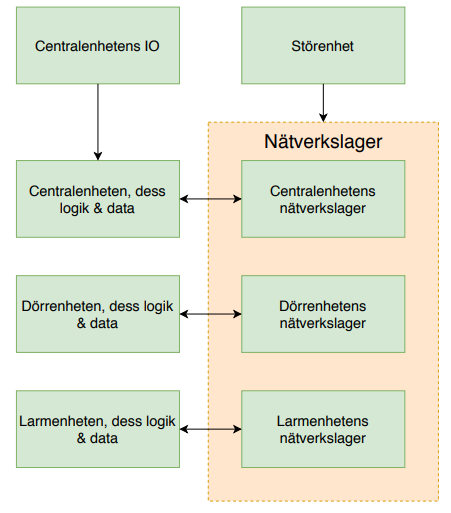
\includegraphics{dokumentation/projektplan/systemoversikt.png}
    \caption{Grafisk representation av systemet}
    \label{fig:systemoversikt}
\end{figure}

\subsubsection{Dörrenheten} 
Dörrenhetens modul ska hålla reda på ifall dörren är öppen eller stängd. Den ska dessutom ha funktioner för att larma ifall dörren har varit öppen längre än en given tid. För att klara av den använder den en dörrsensor. Sensorn kollar dörrens status (öppen, stängd) genom att en ledare med en magnetisk sida sluter en krets då dörren är stängd. Om pull-up motstånd används kommer en 0:a läsas av så länge kretsen är sluten och en 1:a då den är öppen. Hur länge en dörr får stå öppen innan larm skall vara valbart. Dörren ska hålla reda på hur länge sedan sensorn aktiverades och beroende på det utlösa passande larm. Det ska även gå att larma på/av en specifik dörr från centralenheten. 
\newline
\newline
Dörrenheten ska kunna använda nätverkslagret för att ta emot och skicka data till centralenheten. Eftersom att det skall vara möjligt att ha flera dörrar kommer det krävas att varje dörr har ett unik ID. Beslut kommer behöva tas om formatet på ID eftersom att det kommer bestämma hur många dörrar som stöttas. Det valet kommer ta hänsyn till nätverkslagrets begränsningar.

\subsubsection{Larmenheten}
Larmenhetens huvudsakliga uppgift är att utlösa antingen ett ljudbaserat larm eller att tända en varningslampa om rätt krav möts. Dessa krav kan komma från andra moduler t.ex. om dörrsensoren i dörrenheten har varit på för länge eller om larmenheten har tappat kontakt men någon av de andra modulerna. Larmenheten ska också kunna känna av om det sker ett intrång via en ultraljudsbaserad avståndsmätare och en vibrationssensor. 
\newline\newline
Likt dörrenhenten ska det vara möjligt att använda flera larmenheter samtidigt i samma nätverk, det ska också vara möjligt att särskilja vilken larmenhet som utlöser ett larm samt vilken enhet som man vill kommunicera med. Också likt dörrenheten kommer beslut behöva tas angående ID.

\subsubsection{Centralenheten}
\label{sec:centralenhetLD}
Centralenhetens förmåga att bearbeta information är ytterst viktig. Den måste kunna ta emot information från flera sensorer och enheter, till och med samtidigt, och bedöma hur den ska behandla informationen. Den har den viktigaste uppgiften i larmsystemet - att bedöma när larmenheten ska slå larm. 
\newline \newline
Systemet främjas av att information från flera enheter hämtas så snabbt som möjligt. Att använda listor som innehåller referenser till ''structs'' (En datarepresentation av en moduls tillstånd) är därför bra. Centralenheten ska ha en lista med en ''struct'' för varje enhet som är kopplad. Att ha flera moduler av samma typ i listan är möjligt eftersom varje enhet har ett unikt ID. Från denna lista hämtar centralenheten information, och när något behöver konfigureras kan moduler göra ändringarna, och ändra innehållet i sin ''struct'' på förfrågan. 
\newline \newline
En annan viktig användning av listan med moduler är så centralenheten vet att antalet moduler inkopplade inte ändras (utan tillstånd). Genom att ta kontakt och försöka få ett meddelande tillbaka, kan  statuslistan uppdateras, och beroende på hur denna lista ser ut bedömer centralenheten nästa åtgärd. Denna lista med moduler gör det också möjligt för systemet att vara modulärt. 

\subsubsection{Centralenhetens IO}
\label{sec:centralenhetIO}

Centralenheten använder IO enheter keypad, USART och en ljusdiod. Keypad används för att se vilken kod användaren har slagit in för att stänga av larmet vilket sedan skickas vidare till centralenheten som kan se om koden är korrekt. USART används för att ge kommandon och konfigurera centralenheten samt andra moduler. USART kan även användas som en utport där programmet kan skriva ut statusmeddelande för att simplifiera debugging-processen. Ljusdioden aktiveras när systemet larmar lokalt. 
\newline\newline
Eftersom centralenheten tar emot information från flera olika källor är det viktigt att funktionerna som hanterar IO från Keypad och USART kan löpa kontinuerligt.  För att tillåta detta och att alla inmatningar kan registreras och skickas vidare på kort tid kommer ett buffertsystem byggas. Ett buffertsystem hanterar ett inmatat ord genom att lagra endast en bokstav i bufferten innan programmet går vidare för att kolla om det finns indata från andra källor, för att sedan fylla på bufferten tills hela ordet är inmatat. 

\subsubsection{Störenhet}
Störenhetens syfte är att simulera en defekt pereferienhet genom att överflöda de övriga pereferienheterna med stora mängder data för att störa systemet. Mängden data ska vara justerbar för att testa enheternas gränser.

\subsection{Tillägg}
\label{sec:Tillägg}
I mån av tid görs tilläggen. Det distansbaserade larmet prioriteras över larmsignalen.
\subsubsection{Distansbaserat larm}

För att minimera falska larm kommer en avståndsmätare att användas så att det beroende på distans endast larmar lokalt med ljusdioden. Centralenheten larmar endast om objektet vid sensorn rör sig tillräckligt nära. Den maximala distansen ska kunnas konfigureras enkelt vid behov.

\iffalse % upgg 3 beskrivning
Istället för att rörelsesensorn larmar direkt när någon är i närheten skulle
den först kunna larma lokalt ifall någon är inom dess räckvidd, men inte larma till centralenheten förrän
de är inom till exempel en eller två meter. Avståndet ska kunna konfigureras och ni behöver göra tester
för att se hur välkalibrerad ert system är. Tänk på att det här kanske ställer ett högre krav på
noggrannhet i avläsningen av ultraljudssensorn. 
\fi

\subsubsection{Larmsignal}
Ett larmsystems grundläggande funktion är att fånga uppmärksamhet av så många personer som möjligt och det är därför viktigt att välja rätt larmsignal. Konsekvent kommer en signal som höjer sannolikheten att larmet uppmärksammas att väljas.

\iffalse %uppg 8 beskrivning
Extrauppgift 8 (svårighet enkel): En grundprincip för ett larm är att det ska väcka uppmärksamhet när
det larmar. Ett hederspris kommer utdelas till den grupp som har den mest irriterande larmsignalen. 
\fi


\iffalse
För att konkretisera en struktur som ett datorsystem underlättar det
ofta att rita en figur, till exempel ett blockschema, över systemet som
man tänker sig att implementera. I detta avsnitt beskriver ni
översiktligt systemet, lämpligen genom en (eller flera) figur(er). Se
till att hänvisa till figuren från texten och att använda en rubrik för
figuren. Eftersom systemet är ganska komplext behöver ni tänka igenom
vilken detaljrikedom systemöversikten ska ha; dels känner ni ännu inte
till detaljer eftersom konstruktionsarbetet inte påbörjats, dels skulle
inte alla detaljer få plats i en figur över systemet.

I och med att det finns ett grundsystem till vilket man kan lägga
kompletteringar behöver era val av kompletteringar beskrivas
översiktligt. Om ni avser att arbeta med egendefinierade kompletteringar
krävs en mer detaljerad beskrivning än om ni använder kompletteringar
som beskrivs i projektdirektivet.

Under projektets genomförande kommer ni att få anledning att revidera
figuren över systemet. Att ta fram den ultimata figuren över det
slutliga systemet är varken möjligt eller önskvärt under
planeringsfasen, utan det är framförallt processen med att ta fram
figuren som är viktig eftersom denna process hjälper gruppen att
fokusera tänkandet, att skapa gemensamma tekniska ramar och att rensa
bort (en del) tekniska oklarheter.
\fi


\section{Resursplan}
\label{sec:resursplan}

%Gör en lista över gruppmedlemmarna och ange tydligt hur man kommunicerar
%med var och en av dessa (till exempel, ange epostadresser).
%Utgångspunkten är att alla gruppmedlemmar är tillgängliga genom hela
%projektet. Om det finns undantag, ange dessa.
%
%Ange vilka roller som de olika gruppmedlemmarna har. Det är lämpligt att
%en person är ansvarig för ett distinkt område; delat ansvar är
%komplicerat. Här är ett förslag på ansvarsområden inom gruppen. Andra
%områden är möjliga, till exempel kan man dela upp ansvaret för olika
%delar av projektet istället för olika (men var försiktig med det för det
%kan leda till att gruppen blir splittrad). Notera att ansvaret inte
%innebär att man gör mer av det praktiska, snarare att övervakar gruppens
%arbete och uppmärksammar gruppen när något inte fungerar.

%\begin{itemize}
%    \item Gruppledare: Ansvarar för kommunikation med kursens lärare, ansvarar
%    för att kalla till och leda gruppmöten.
%
%    \item Administrativt dokumentationsansvarig: Ansvarar för att
%    mötesprotokoll förs. Ansvarar för att gruppen i tid börjar på
%    oppositionsrapport, planeringsrapport och så vidare och ansvarar för
%    att dessa skickas in i tid.
%
%    \item Teknisk dokumentationsansvarig: Ser till att kod är väl kommenterad.
%    Uppmärksammar gruppen ifall det uppstår problem med kod som inte är
%    tillräckligt dokumenterad.
%
%    \item Kodstandardansvarig: Kollar igenom att all kod som utvecklas följer
%    standarder för struktur, namn och så vidare som gruppen bestämt.
%    Uppmärksammar gruppen ifall disciplinen behöver skärpas vad
%    gäller kodkvalitet.
%
%    \item Testansvarig: Håller ordning på de olika test som behöver genomföras
%    på mjukvara och hårdvara, ser till att tillräcklig tid ägnas åt
%    testning och att den dokumenteras väl. Uppmärksammar gruppen ifall
%    testningen inte utförs eller dokumenteras tillräckligt.
%
%    \item Resursansvarig: Ser till att hårdvaran finns tillgänglig när den
%    behövs, ansvarar för att olika verktyg ni använder för
%    kommunikation, versionshantering och så vidare fungerar och
%    används korrekt. Uppmärksammar gruppen ifall verktygen används fel
%    eller inte fungerar väl.
%
%    \item Planeringsansvarig: Håller reda på de olika del-mål gruppen arbetar
%    mot, kommunicerar med de andra gruppmedlemmarna om hur arbetet med
%    dessa fortskrider och ger en rapport om det på veckomöten.
%    Uppmärksammar gruppen så tidigt som möjligt om något mål inte gör
%    framsteg så att gruppen kan planera om ifall det behövs eller så att
%    arbetsinsatser kan omfördelas.
%
%\end{itemize}
%
%Ange vilka lokaler som kan disponeras, och när. Ange vilken hårdvara och
%vilken mjukvara som finns tillgänglig. I och med att en del hårdvara
%görs tillgänglig på begäran, ange hur ni begär ut hårdvara.
%
%Om gruppmedlemmar vill arbeta med projektet på distans, utanför
%Chalmers, beskriv hur man lämpligen går tillväga.

Nedan följer en lista av gruppens alla medlemmar, deras e-postadresser samt
ansvarsområde som delades ut under gruppmöte \#1. Utöver detta har även en
discord-kanal och en messenger-grupp skapats för kommunikation inom gruppen.
\begin{table}[h]
\resizebox{\textwidth}{!}{%
\begin{tabular}{ | l | l | l | }
\hline
  \thead{Namn} & \thead{e-post}  & \thead{ansvarsområde}  \\
\hline\hline
 Felix Bråberg & braberg.felix@gmail.com & \makecell{Gruppledare \\ Centralenhetens nätverkslager} \\
\hline
 Erik Nilsson & ernilsso@net.chalmers.se   & \makecell{Administrativ dokumentationsansvarig\\Dörrenhetens logik och data} \\
\hline
 Sebastian Sjögren & sebastiansjogrn@gmail.com & \makecell{Teknisk dokumentationsansvarig \\ Centralenhetens inmatning}  \\
\hline
 Gabriel Käll & gabbekall@gmail.com & \makecell{Kodstandardansvarig \\ Centralenhetens logik och data}  \\
\hline
 Linus Haraldsson & linusharaldsson00@gmail.com & \makecell{Testansvarig \\ Larmenhetens Nätrverkslager} \\
\hline
Simon Widerberg & widerbergsimon@gmail.com & \makecell{Resursansvarig \\ Larmenhetens logik och data} \\
\hline
Philip Antonsson & phiant@student.chalmers.se & \makecell{Planeringsansvarig \\ Dörrenhetens nätverkslager}  \\
\hline
\end{tabular}}
\caption{Gruppmedlemmar med tillhörande information}
\label{Tabell medlemmar}
\end{table}

Lokaler som kan användas är rum 4211(där hårdvaran förvaras), detta rummet kan
bokas enligt anvisningar på Canvas “Bokning av arbetsrum”. Utöver detta kan
även Chalmers vanliga grupprum användas och bokas. Om man vill arbeta på
distans kan man använda sig av gruppens GitHub för att pusha och pulla
ändringar, alltså lägga upp ändringarna som gjorts på GitHub och hämta ändringar som andra laddat upp. Om man behöver hjälp eller har en fråga kan man kontakta de
andra gruppmedlemmarna så som nämnts ovanför, vi har även planerat in att arbeta en del på
distans med hjälp av Discord och dylikt. Mjukvara som kan utnyttjas är codelite
för kodskrivande i språket C. Hårdvaran som är tillgänglig finns i rum
4211 i skåpet med kod 3542 och är som följer:
\newpage
\begin{table}[h]

\begin{tabular}{ | l | l | l | }
\hline
Antal & Enhet  & Plats \\
\hline\hline
3 & MD407 kort & Kassaskåpet \\
\hline
1 & Avståndsmätare (ultraljud), HC-SR04 & Kassaskåpet \\
\hline
1  & Vibrationssensor, "Flying-Fish" SW-18010P & Kassaskåpet  \\
\hline
1  & Keypad & Kassaskåpet  \\
\hline
1 &7-segmentsdisplay  & Kassaskåpet \\
\hline
2 & 4-polig RJ-11 kabel (för CAN-bussen)& Kassaskåpet \\
\hline
1 & RJ-11 förgrening & Kassaskåpet \\
\hline
2 & Tiopolig flatkabel & Kassaskåpet \\
\hline
3 & USB-kabel & Kassaskåpet \\
\hline
1 & Kopplingsplatta & Kassaskåpet \\
\hline
N/A & Kopplingskablar & Kassaskåpet \\
\hline
N/A & Dörrsensor  & Fråga handledare \\
\hline

\end{tabular}
\caption{Hårdvara och plats den kan hittas samt antal}
\label{Tabell hardvara}
\end{table}

\section{Milstolpar}
\label{sec:milstolpar}

{
\begin{table}[ht]
    \centering
    \resizebox{\columnwidth}{!}{
    \begin{tabular}{|c|c|c|c|}
         \hline
         Läsvecka & Datum & Typ & Händelse \\
         
         \hline\hline
                      2 & 2020-09-11 & Mål & Konfigurera/synka GIT \\
                      & 2020-09-11 & Mål & Testa Hårdvara \\
                      & 2020-09-13 & Inlämning & Projektplan \\
                      
         \hline\hline
                      3 & 2020-09-14 & Mål & Påbörja rapporten \\
                      & 2020-09-15 & Mål & Påbörja projektet \\
         
         
         \hline\hline
                      4 & 2020-10-02 & Mål & Grundsystem klar för granskning \\
                      & 2020-10-04 & Inlämning & Rapportutkast 1 \\
                      
         \hline\hline
                      5 & 2020-10-08 & Inlämning & Oppositionsrapport \\
                      & 2020-10-09 & Mål & Kod klar och granskad \\
                      & 2020-10-09 & Mål & Extrauppgift 3 Klar \\
                      & 2020-10-09 & Mål & Extrauppgift 8 \\
                      
         \hline\hline
         7 & 2020-10-18 & Inlämning & Rapportutkast 2 \\
         
         \hline\hline
         8 & 2020-10-28 & Mål & All kodning klar \\
         
         \hline\hline
                      9 & 2020-11-01 & Inlämning & Slutrapport \\
                      & 2020-11-01 & Inlämning & Medverkansrapport \\
                      & TBD & Inlämning & Demo \\
                      
         \hline
    \end{tabular}}
    \caption{Milstolpar för projektet}
    \label{tab:milstolpar}
\end{table}
}

\section{Aktiviteter}
\label{sec:aktiviteter}
\iffalse
Här ger ni en detaljerad beskrivning av arbetspaket/arbetsuppgifter
kopplat till total tidsåtgång per paket. Tidsåtgången är alltså inte per
medlem utan det är en total siffra (“mantimmar”) för alla som är
involverade i just denna aktivitet. En kurs om 7,5 p motsvarar ju 200
timmar per student. I grupper om sju eller åtta personer finns det
alltså totalt 1400 eller 1600 timmar att disponera till olika
aktiviteter.

När ni sitter och skriver på denna lista vet ni ju exakt hur många
timmar som redan använts (och ja, dessa timmar ska också skrivas ned!)
men för veckorna framgent måste ni gissa. Ett exempel på de första
raderna i en aktivitetslista ges i tabell [tab:aktiviteter].
\fi
En kurs på 7,5hp täcker 200h.
I tabellen \ref{tab:aktiviteter} anges hur vi har valt att dela upp tiden.
Bemärk att tabellen endast innehåller 1337h. Varje medlem har då 9h extra att lägga skulle det behövas.
\newpage
\begin{table}[h]
    \centering
    \begin{tabular}{l|l|l}
         Aktivitet & Tid(h) & Deltagande \\
         \hline
         Planeringsrapport & 149 & Alla \\
         Veckomöten & 112 & Alla \\
         Möten & 128 & Alla\\
         Demo + förberedelser & 28 & Alla \\
         Övning 1 & 14 & Alla \\
         Övning 2& 8 & Philip, Erik, Linus, Simon \\
         Övning 3& 14 & Alla \\
         Oppositionsrapport & 28 & Alla \\
         Arbete med projektrapport & 489 & Alla \\
         Modul, dörrenhet & 42 & Philip, Erik \\
         Modul, larmenhet & 42 & Linus, Simon \\
         Modul, centralenhet & 42 & Felix, Sebastian, Gabriel \\
         Nätverkslager & 60 & Philip, Linus, Felix  \\
         Störenhet & 8 & Linus \\
         Extra uppgift 3 & 24 & Alla \\
         Extra uppgift 8 & 6 & Alla\\
         Dokumentgranskning& 21 & Alla \\
         Projektledning &  24 & Felix \\
         Insättning i hårdvaran & 42 & Alla \\
         Dokumentation läsning & 42 & Alla\\
         Kamratuppskattning och medverkans-rapport & 14 & Alla\\
         Utforming av konventioner & 5 & Gabriel\\
         \hline
    \end{tabular}
    \caption{Aktivitetstabell över förväntat arbete}
    \label{tab:aktiviteter}
\end{table}

\iffalse
  : Aktivitetslista för projektet

Eftersom ni förr eller senare ska matcha aktiviteter till medlemmar är
ett tips att ni skriver upp vilken eller kanske snarare vilka
gruppmedlemmar som hör ihop med respektive aktivitetet. Med denna
planering blir det sedan möjligt för gruppen att följa upp arbetet i de
veckovisa projektgruppsmötena.
\fi


\section{Tidsplan}
\label{sec:tidsplan}
Arbetets planering redovisas här med hjälp av ett gantschema. Se figur \ref{fig:sept1} och \ref{fig:sept2} samt \ref{fig:oct1} och \ref{fig:oct2} för Semptembers respektive Oktobers tidsplan. 

\begin{figure}[h]
    \centering
    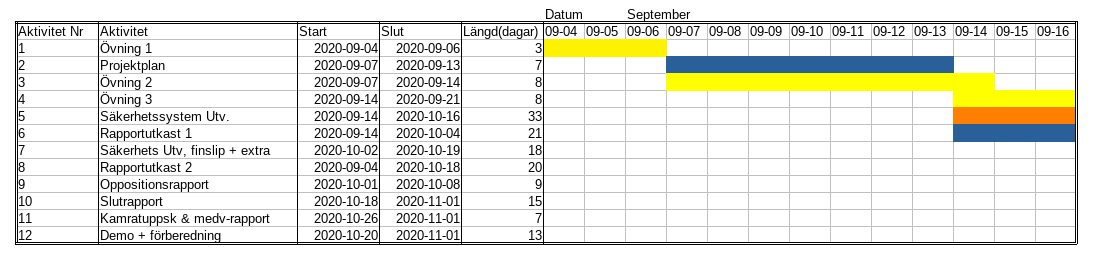
\includegraphics[scale=0.44, angle=0]{dokumentation/projektplan/september1.png}
    \caption{En ganttbaserad tidsplan för första halvan av September.}
    \label{fig:sept1}
\end{figure}

\begin{figure}[h]
    \centering
    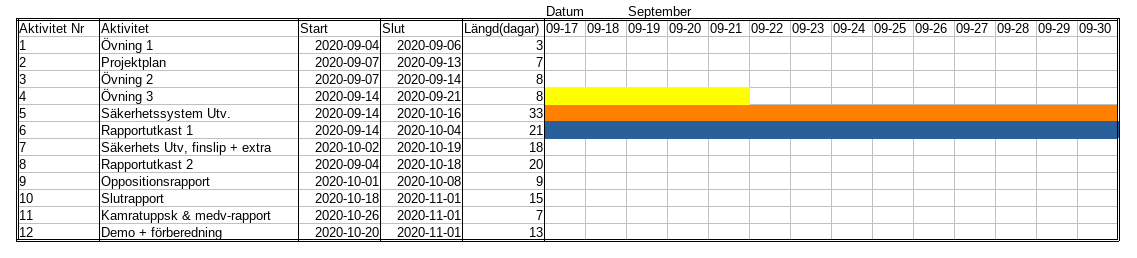
\includegraphics[scale=0.44, angle=0]{dokumentation/projektplan/september2.png}
    \caption{En ganttbaserad tidsplan för andra halvan av September.}
    \label{fig:sept2}
\end{figure}
\newpage
\begin{figure}[h]
    \centering
    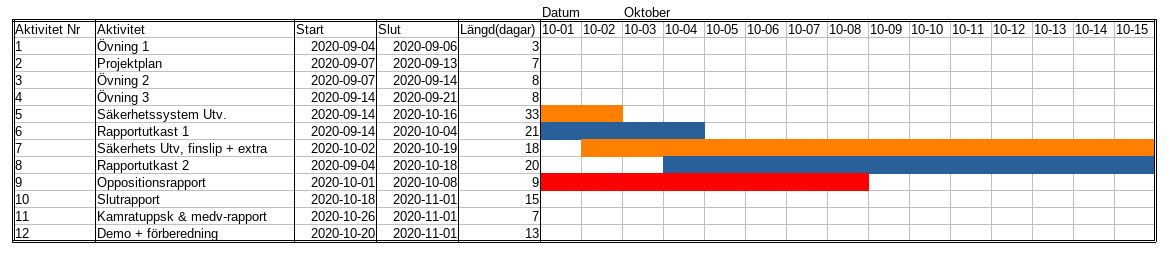
\includegraphics[scale=0.43, angle=0]{dokumentation/projektplan/oktober1.png}
    \caption{En ganttbaserad tidsplan för första halvan av Oktober.}
    \label{fig:oct1}
\end{figure}

\begin{figure}[h]
    \centering
    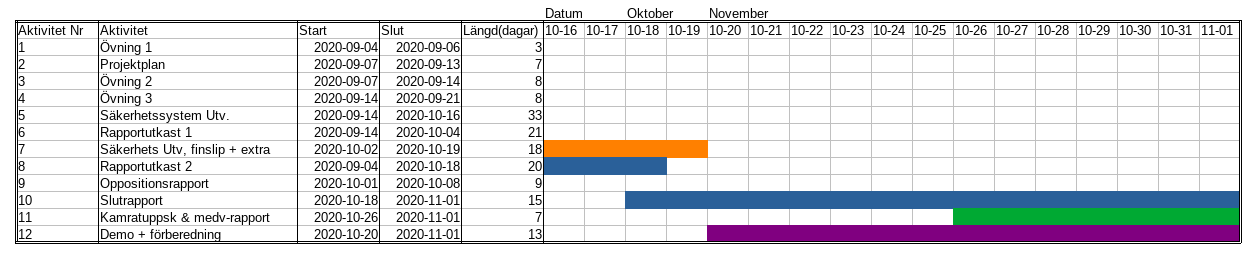
\includegraphics[scale=0.36, angle=0]{dokumentation/projektplan/oktober2.png}
    \caption{En ganttbaserad tidsplan för andra halvan av Oktober.}
    \label{fig:oct2}
\end{figure}

\iffalse
Det kommer periodvis att finnas flera olika aktiviteter som löper
parallellt. Ta till exempel läsvecka 7 och 8 där 1) en
oppositionskommentar för en annan grupps projektrapportsutkast ska
skrivas, 2) en demonstration av slutprodukten ska förberedas och
genomföras, och 3) en projektrapport v. 1 ska avslutas. Med en grupp om
sju-åtta personer bör man planera så att dessa aktiviteter på ett
smidigt sätt löper parallellt. Ett Ganttschema (se figur \ref{fig:sept}) samt
\ref{fig:oct}
kan illustrera de olika aktiviteterna (och möjligen även milstolparna)
på en horisontell tidslinje.


Om man kan koppla de olika aktiviteterna till gruppmedlemmar (risken
finns att Ganttschemat kan bli rörigt) finns det en möjlighet att
urskilja kritiska beroenden mellan olika delar av projektet.
\fi

\section{Mötesplan}
\label{sec:mötesplan}
\iffalse
Beskrivning:
Ange datum, tid och lokal för de veckovisa projektmötena som involverar
hela gruppen samt handledare. Ange även, så långt det är möjligt, datum,
tid och lokal för mer specialiserade arbetsmöten.
\\
\\
\fi
Med åtanke till rådande omständigheter gällande covid-19 har gruppen valt att i förstahand ha möten på distans.
Praktiska moment som kräver fysisk närvaro gör dock på plats.
En delad kalender används för att enas, och påmminnas, om vilka möten, tider och deadlines som behöver passas.
\newline
\newline
Det ska hållas veckliga möten med handledaren, Rasmus Edvardsson, på onsdagar kl:14-15. Med undantag onsdag den nionde september då den är kl:9-10. De mötena kommer ta plats i zoom. Länken utges av gruppledaren, Felix Bråberg, i kallelsen som ska komma senast två dagar innan planerat möte. Målet är att inte ändra tider, det är upp till gruppens medlemar att ha tiden fri. Tider kan dock ändras för att säkra handledarens närvaro.
\newline
\newline
Arbetsmöten kommer också att ske på tisdagar, torsdagar och fredagar. De sker i röstsamtal på Discord klockan 13.15-15. I det fall att övningspass sammanfaller prioriteras den. Det finns tider när handledarna är tillgängliga för frågor och konsultation på zoom. Under arbetspassen och veckomötet bestämms det ifall gruppen som helhet har behov att närvara. 


\section{Kommunikationsplan}
\label{sec:kommunikationsplan}

Här ses en full tabell av alla planerade kommunikationsmoment.

%\newpage % kan behövas om tabellstorlek krånglar, annars kan longtable funka men det är också konstigt.

\iffalse %sätt att blockkommentera i latex, false->true tar bort kommentar
Det blir en hel del skrivande i ett projekt. För större projekt är
kommunikationen så komplex att det är värt att tydligt definiera en plan
över all skriftlig kommunikation. Man kan exempelvis presentera det som
i tabell \ref{tab:kommunikationsplan} (där PP står för PingPong, och Alla
betyder grupp, mentor och lärarteam).

Här har jag utgått från att det finns 1) en dokumentationsansvarig som
ser till att dokument som projektplan och projektrapport i rätt tid
sänds till rätt adressat och 2) en projektledare som ser till att
dagordning och mötesprotokoll läggs upp på PingPong.
\fi
{
\begin{table}[ht]
    \centering
    \resizebox{\columnwidth}{!}{
    \begin{tabular}{|c|c|c|c|}
         \hline
         Vad & När & Till & Hur \\ [0.5ex]
         \hline\hline
         Planering projektplan & 2020-09-07 & Grupp & Discord \\
         \hline
         Fjärrarkiv & 2020-09-09 & Handledare & Github\\
         \hline
         Veckoschema & 2020-09-09 & Handledare & Zoom\\
         \hline
         Preliminär projektplan & 2020-09-10 & Grupp & Github  \\
         \hline
         Projektplan & 2020-09-11 & Lärarteam & Canvas inlämning  \\
         \hline
         Rapportutkast & 2020-10-04 & Lärarteam & Canvas inlämning  \\
         \hline
         Oppositionsrapport & 2020-10-08 & Lärarteam & Canvas inlämning  \\
         \hline
         Rapportutkast 2 & 2020-10-18 & Lärarteam & Canvas inlämning  \\
         \hline
         Demo & Vecka 9 & Lärarteam & Canvas inlämning  \\
         \hline
         Slutrapport & 2020-11-01 & Lärarteam & Canvas inlämning  \\
         \hline
         Medverkandesrapport & 2020-11-01 & Lärarteam & Canvas inlämning  \\
         \hline
    \end{tabular}
    }
    \caption{Kommunikationsplan för projektet}
    \label{tab:kommunikationsplan}
\end{table}
}
Ovanpå denna tabell hålls ett möte på zoom med handledare Rasmus Edvardson på onsdag varje vecka. Det kommuniceras även ett mötesprotokoll samma dag varje vecka efter utfört formellt möte. Mötesprotokollet skickas genom canvas till arbetsgruppens handledare.\\

Gruppen har planerat att använda discord och messenger som sin huvudsakliga kommunikationsmetod mellan varandra medan canvas och zoom används för inlämningar och konversationer med lärarteam och handledare. 

\iffalse
Se även till att ni tidigt enas om hur ni kommunicerar inom gruppen:
Ni har visserligen tillgång till en grupplogg inom PingPong där ni kan
beskriva era framsteg, men ni behöver dessutom ha någon slags
peer-to-peer-kommunikation.
\fi

\section{Kvalitetsplan}
\label{sec:kvalitesplan}

All kod ska följa den överenskomna kodkonventionen för en konsekvent kod. Dessutom behöver all kod bli godkänd av en annan gruppmedlem innan den flyttas från utvecklingsmiljön till den slutliga versionen. Testansvarig, Linus Haraldsson, ser till att alla tester utförs, men varje gruppmedlem ansvarar för att utföra tester på den komponent de utvecklar.
\newline
\newline
Vid verifiering av ett delsystem ska mallen nedan kortfattat fyllas i för att strukturerat utföra alla tester som krävs och kommunicera vad som behöver åtgärdas. Dessutom blir det därefter tydligt vart det krävs yttligare tester. Testdokumentation ska samlas under mappen “test\_dokument” på GitHub.
\newline
\newline
\newline
\newline
\subsection*{Mall för testdokumentation}
\begin{description}
    \item[Komponent]{Vilken del av system ska testas? Hårdvara eller mjukvara?}
    \item[Testsyfte]{Vad ska testet visa? Vilka scenarior är det som faktiskt testas?}
    \item[Hypotes]{Vad förväntas av testets resultat? }
    \item[Utförande]{Hur ska testet utföras? Förklara stegvis om det behövs.}
    \item[Resultat]{Endast testets resultat }
    \item[Analys]{Vad innebär testets resultat?  }
    \item[Övrigt]{Vad mer behöver testas? }
    
\end{description}

\iffalse
Beskriv era rutiner för att verifiera respektive delsystem och, i
slutändan, hela systemet. Ni kan till exempel använda en enkel
verifieringsmall som ska fyllas i samband med att en del av systemet
verifieras: Här kan man tänka sig rubriker som

Tänk på att olika delar av systemet behöver olika verifieringsmetodik;
medan mjukvara kan verifieras i det IDE (Integrated Design Environment)
som ni använder, behöver ni använda mätutrustning för elektronik.
\fi

\section{Spelregler}
\label{sec:spelregler}

Bestämda spelregler består av följande:

\begin{itemize}
\item Inget grupparbete under helg eller efter klockan 5 då alla gruppmedlemar inte är tillgängliga. Enskilda gruppmedlemar kan dock arbeta vid frivillig tid. 
\item Allt planerat arbete ska inlämnas innan bestämd tid.
\item Alla gruppmedlemar förväntas att aktivt ta del i arbetet och göra de uppgifter gruppen har tilldelat dem.
\item Vid misslyckande att följa spelregler hålls ett gruppmöte där konsekvenserna till arbetet observeras och åtgärder bestäms för att lösa konsekvenserna.
\end{itemize}
\iffalse
Denna rubrik kring spelregler är helt frivillig eftersom den normalt
sett inte ingår i en projektplan. Skälet för att ha med spelregler här
är att göra er överenskommelse kring dessa synlig och tydlig. Följden är
att att ingen gruppmedlem senare kan säga att han eller hon inte är
införstådd med dessa. Det kan handla om någonting så simpelt som vad
konsekvensen är av att någon kommer för sent till ett möte. Men det kan
också handla om mer allvarliga saker som att någon enskild medlem inte
levererar material vid en tidpunkt som gruppen bestämt i projektplanen.
\fi

\bibliographystyle{IEEEtran}
\bibliography{referenser}
\end{document}
